\documentclass[paper=a4, 
                DIV=12]{scrartcl}
\usepackage[ngerman]{babel} % Deutsche Sprache
\usepackage[utf8]{inputenc}
\usepackage{graphicx} % Required for inserting images
\usepackage{matlab-prettifier}
\usepackage{amsmath}
\usepackage{float}

\title{MatLab Programmentwurf}
\author{Timo Johannsen, Benjamin Peiter, Omer Butt}
\date{27. April 2025}

\begin{document}

\maketitle
\newpage
\tableofcontents
\newpage

\section{Visualisierung der Systemdynamik durch Phasenportraits}
Zuerst werden 3 verschiedene K-Werte mit $K_{1} = ]0,0.6]$, $K_{2} = [0.9,1.1]$ und \hbox{$K_{3} = [1.4,2.0]$} gewählt und die Länge und Anzahl der Trajektorien definiert. 
\begin{lstlisting}[frame=single, style=Matlab-editor]
K_values = [rand()*0.6, 0.9 + rand()*0.2, 1.4 + rand()*0.6];
    % Parameter fuer die drei K-Werte
N = 1000; % Laenge der Trajektorien
M = 50; % Anzahl der Trajektorien
\end{lstlisting}
Daraufhin werden für die 3 K-Werte die Phasenportraits erstellt. In einer Schleife werden durch die K-Werte iteriert und für jeden K-Wert die Trajektorien gezeichnet.
\begin{lstlisting}[frame=single, style=Matlab-editor]
figure;
for idx = 1:3
    K = K_values(idx);
    subplot(1,3,idx);
    hold on;
\end{lstlisting}
Jede Trajektorie bekommt eine zufälligen Startpostition $(I_0, \theta_0)$ aus dem Bereich \hbox{$[0,2\pi]$ x $[0,2\pi]$}.
Zusätzlich wird für die Trajektorie zwei Vektoren der Länge 1000 erstellt, in der die Werte für $I$ und $\theta$ gespeichert werden.
\begin{lstlisting}[frame=single, style=Matlab-editor]
    for m = 1:M
        I = rand()*2*pi;
        theta = rand()*2*pi;
        I_traj = zeros(1,N);
        theta_traj = zeros(1,N);
\end{lstlisting}
Die Trajektorie wird dann rekursiv berechnet. Dabei werden die Formeln:
\begin{gather*}
    I_{n+1} = (I_n + K \cdot \sin(\theta_n)) \bmod 2\pi \\
    \theta_{n+1} = (\theta_n + I_n) \bmod 2\pi
\end{gather*}
verwendet, wobei $I$ und $\theta$ in jedem Schritt aktualisiert werden. Die Trajektorie wird dann in den Vektoren gespeichert und zum Schluss wird jeder Punkt gezeichnet.
\begin{lstlisting}[frame=single, style=Matlab-editor]
        for n = 1:N
            I = mod(I + K*sin(theta), 2*pi);
            theta = mod(theta + I, 2*pi);
            I_traj(n) = I;
            theta_traj(n) = theta;
        end
        plot(theta_traj, I_traj, '.', 'MarkerSize', 1);
    end
\end{lstlisting}
Diese Werte werden dann in einem Diagramm gezeichnet. Dabei wird die x-Achse mit $\theta$ und die y-Achse mit $I$ beschriftet.
\newpage
\noindent Dabei charakterisieren die Phasenportraits die Dynamik des Systems, dass für ein wachsendes K das chaotische Verhalten zunimmt. \\
\begin{figure}[H]
    \centering
    \begin{minipage}[t]{0.48\textwidth}
        \centering
        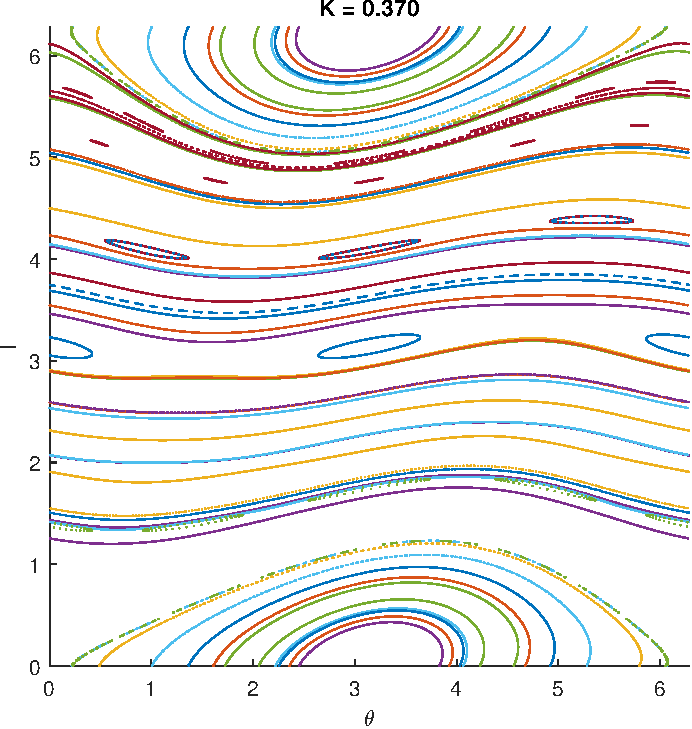
\includegraphics[height=0.33\textheight]{phasenportrait_k1.pdf}
        \caption{Phasenportrait für $K_1$}
    \end{minipage}
    \hfill
    \begin{minipage}[t]{0.48\textwidth}
        \centering
        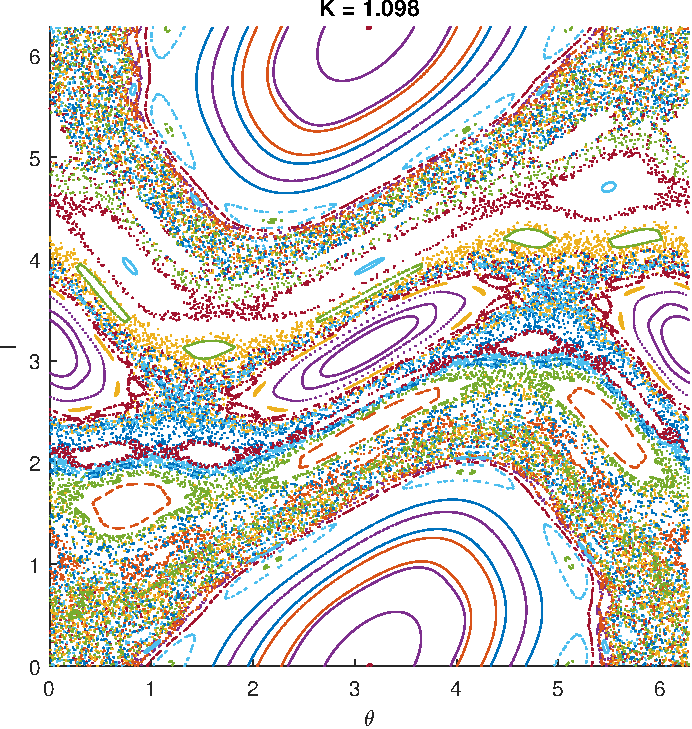
\includegraphics[height=0.33\textheight]{phasenportrait_k2.pdf}
        \caption{Phasenportrait für $K_2$}
    \end{minipage}
    \par\vspace{1.3cm}
    \begin{minipage}[t]{0.48\textwidth}
        \centering
        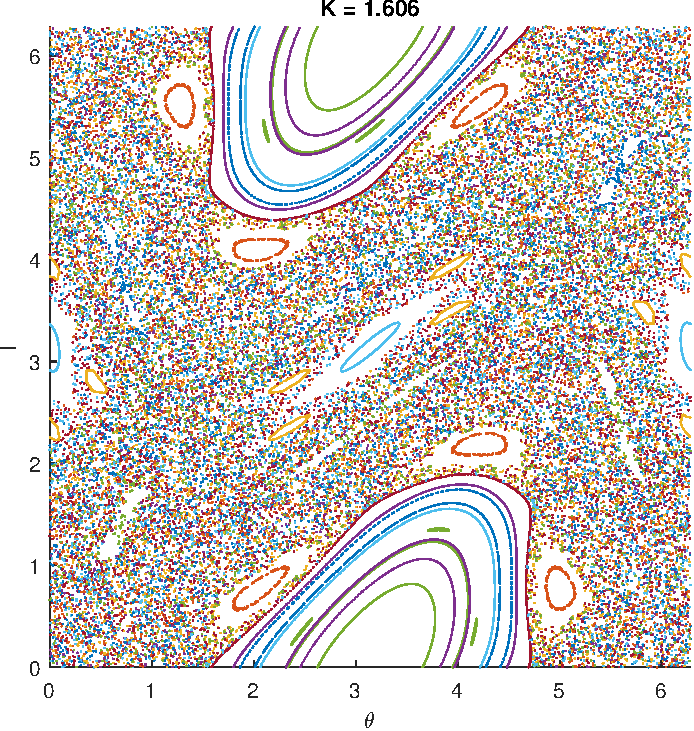
\includegraphics[height=0.33\textheight]{phasenportrait_k3.pdf}
        \caption{Phasenportrait für $K_3$}
    \end{minipage}
\end{figure}

\newpage
\section{Quantifizierung des Chaos durch Ljapunov-Exponenten}

\begin{lstlisting}[frame=single, style=Matlab-editor]
K_vals = linspace(0, 4, 200);
N = 1000;
lambda1 = zeros(size(K_vals));
lambda2 = zeros(size(K_vals));

for idx = 1:length(K_vals)
    K = K_vals(idx);
    I = rand()*2*pi;
    theta = rand()*2*pi;
    Q = eye(2);
    sum_log_diag = zeros(1,2);

    for n = 1:N
        I = mod(I + K*sin(theta), 2*pi);
        theta = mod(theta + I, 2*pi);
        % Ableitungsmatrix DF
        DF = [1, K*cos(theta); 1, 1 + K*cos(theta)];
        A = DF * Q;
        [Q, R] = qr(A);
        sum_log_diag = sum_log_diag + log(abs(diag(R))');
    end

    lambda1(idx) = sum_log_diag(1)/N;
    lambda2(idx) = sum_log_diag(2)/N;
end
\end{lstlisting}

\end{document}
